% Fig. 1 of the NTAR manuscript: the evaluated system only (NTAR / NTAR-R).
% Compile with: pdflatex fig1_architecture.tex  ->  fig1_architecture.pdf
\documentclass[border=3pt]{standalone}
\usepackage{times}
\usepackage{amsmath,amssymb}
\usepackage{tikz}
\usetikzlibrary{arrows.meta,calc,backgrounds}

\definecolor{ink}{HTML}{1F1F1E}
\definecolor{muted}{HTML}{5F5E58}
\definecolor{line}{HTML}{8A8A85}
\definecolor{orange}{HTML}{EB6834}
\definecolor{green}{HTML}{1BAF7A}
\definecolor{greenbg}{HTML}{E8F6EF}
\definecolor{redbg}{HTML}{FCEBE4}
\definecolor{bluebg}{HTML}{EAF2FC}
\definecolor{panel}{HTML}{F4F4F1}

\begin{document}
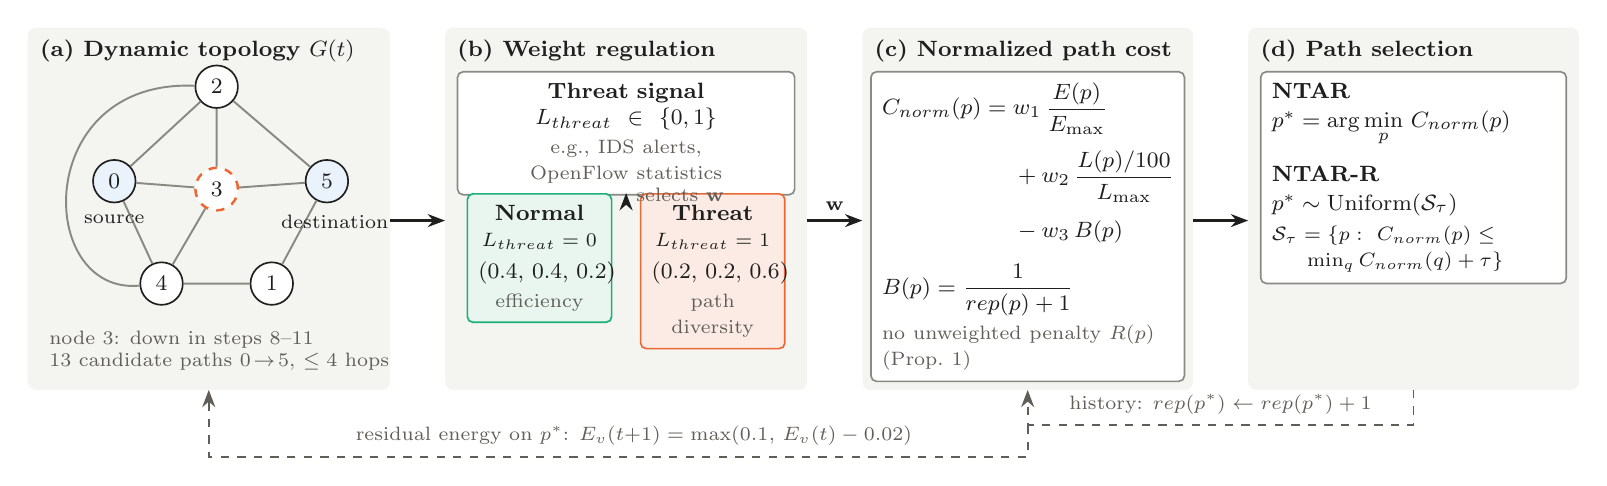
\begin{tikzpicture}[
  font=\footnotesize, text=ink,
  >={Stealth[length=2.2mm]},
  vtx/.style={circle, draw=ink, fill=white, line width=0.6pt, minimum size=5.4mm, inner sep=0pt},
  edge/.style={draw=line, line width=0.7pt},
  card/.style={draw=line, rounded corners=2pt, line width=0.6pt, fill=white, inner sep=4pt},
  flow/.style={->, draw=ink, line width=0.8pt},
  fb/.style={->, draw=muted, line width=0.7pt, dashed},
  ttl/.style={font=\footnotesize\bfseries, anchor=north west, inner sep=0pt},
]
% ---------------------------------------------------------------- panel backgrounds
\fill[panel, rounded corners=3pt] (0,0) rectangle (4.6,4.6);
\fill[panel, rounded corners=3pt] (5.3,0) rectangle (9.9,4.6);
\fill[panel, rounded corners=3pt] (10.6,0) rectangle (14.8,4.6);
\fill[panel, rounded corners=3pt] (15.5,0) rectangle (19.7,4.6);
\node[ttl] at (0.15,4.45) {(a) Dynamic topology $G(t)$};
\node[ttl] at (5.45,4.45) {(b) Weight regulation};
\node[ttl] at (10.75,4.45) {(c) Normalized path cost};
\node[ttl] at (15.65,4.45) {(d) Path selection};

% ---------------------------------------------------------------- (a) topology
\begin{scope}[shift={(0.55,1.1)}]
  \node[vtx, fill=bluebg] (n0) at (0.55,1.55) {0};
  \node[vtx] (n2) at (1.85,2.75) {2};
  \node[vtx, draw=orange, dashed, line width=0.9pt] (n3) at (1.85,1.45) {3};
  \node[vtx, fill=bluebg] (n5) at (3.25,1.55) {5};
  \node[vtx] (n4) at (1.15,0.25) {4};
  \node[vtx] (n1) at (2.55,0.25) {1};
  \draw[edge] (n0)--(n2) (n0)--(n3) (n0)--(n4) (n2)--(n3) (n2)--(n5)
              (n3)--(n5) (n3)--(n4) (n4)--(n1) (n1)--(n5);
  \draw[edge] (n2) .. controls (-0.5,2.85) and (-0.45,0.1) .. (n4);
  \node[font=\scriptsize, anchor=north] at ($(n0.south)+(0,-0.02)$) {source};
  \node[font=\scriptsize, anchor=north] at ($(n5.south)+(0.1,-0.02)$) {destination};
\end{scope}
\node[font=\scriptsize, text=muted, align=left, anchor=south west] at (0.15,0.12)
  {node 3: down in steps 8--11\\13 candidate paths $0\!\to\!5$, $\le 4$ hops};

% ---------------------------------------------------------------- (b) weights
\node[card, text width=4.0cm, align=center, anchor=north] (thr) at (7.6,4.05)
  {\textbf{Threat signal} $L_{threat}\in\{0,1\}$\\[1pt]
   {\scriptsize\color{muted}e.g., IDS alerts, OpenFlow statistics}};
\node[card, fill=greenbg, draw=green, text width=1.55cm, align=center, anchor=north] (nom) at (6.5,2.5)
  {\textbf{Normal}\\{\scriptsize $L_{threat}=0$}\\[2pt]$(0.4,\,0.4,\,0.2)$\\[1pt]{\scriptsize\color{muted}efficiency}};
\node[card, fill=redbg, draw=orange, text width=1.55cm, align=center, anchor=north] (thw) at (8.7,2.5)
  {\textbf{Threat}\\{\scriptsize $L_{threat}=1$}\\[2pt]$(0.2,\,0.2,\,0.6)$\\[1pt]{\scriptsize\color{muted}path diversity}};
\draw[flow] (thr.south) -- (nom.north -| thr.south) node[pos=0.45, right, font=\scriptsize, text=muted] {selects $\mathbf{w}$};

% ---------------------------------------------------------------- (c) cost
\node[card, text width=3.7cm, align=left, anchor=north] (cost) at (12.7,4.05)
  {$\displaystyle
   \begin{aligned}
   C_{norm}(p) ={}& w_1\,\frac{E(p)}{E_{\max}}\\[2pt]
              & + w_2\,\frac{L(p)/100}{L_{\max}}\\[2pt]
              & - w_3\,B(p)
   \end{aligned}$\\[6pt]
   $\displaystyle B(p)=\frac{1}{rep(p)+1}$\\[2pt]
   {\scriptsize\color{muted}no unweighted penalty $R(p)$ (Prop.~1)}};

% ---------------------------------------------------------------- (d) selection
\node[card, text width=3.6cm, align=left, anchor=north] (sel) at (17.6,4.05)
  {\textbf{NTAR}\\[1pt]
   $p^*=\displaystyle\arg\min_{p}\, C_{norm}(p)$\\[6pt]
   \textbf{NTAR-R}\\[1pt]
   $p^*\sim\mathrm{Uniform}(\mathcal{S}_\tau)$\\[3pt]
   {\scriptsize $\mathcal{S}_\tau=\{p:\ C_{norm}(p)\le{}$\\\hspace*{1.6em}$\min_q C_{norm}(q)+\tau\}$}};

% ---------------------------------------------------------------- main flow
\draw[flow] (4.6,2.15) -- (5.3,2.15);
\draw[flow] (9.9,2.15) -- node[above, font=\scriptsize] {$\mathbf{w}$} (10.6,2.15);
\draw[flow] (14.8,2.15) -- (15.5,2.15);

% ---------------------------------------------------------------- feedback
\draw[fb] (17.6,0) -- (17.6,-0.45) -- (12.7,-0.45) -- (12.7,0);
\node[font=\scriptsize, text=muted, anchor=south] at (15.15,-0.43) {history: $rep(p^*)\leftarrow rep(p^*)+1$};
\draw[fb] (12.7,-0.45) -- (12.7,-0.85) -- (2.3,-0.85) -- (2.3,0);
\node[font=\scriptsize, text=muted, anchor=south] at (7.7,-0.83)
  {residual energy on $p^*$: $E_v(t{+}1)=\max(0.1,\,E_v(t)-0.02)$};
\end{tikzpicture}
\end{document}
